\documentclass[10pt]{article}
\usepackage[margin=0.7in]{geometry}
\usepackage{graphicx,booktabs,hyperref,amsmath}
\hypersetup{colorlinks=true,urlcolor=blue}
\setlength{\parindent}{0pt}
\setlength{\parskip}{6pt}
\title{Quadratic-twist evidence import and native audit}
\author{Reproducible study record}
\date{21 October 2026}
\begin{document}
\maketitle
\vspace{-1em}
\textbf{Scope.} Import the prior experiment records into \texttt{aburan28/crypto}.
The frozen source and original records remain historical Python evidence. A new
C++17 auditor verifies a declared subset independently. This is not a full native
port, a performance comparison, or a general ECDLP hardness result.

\textbf{Historical record.} The completed run records 942 nonsingular curve
models over primes 5, 7, 11, 13, 17, 19; 4,188,162 ordered S3 triples;
113,342 ordered S4 quadruples over primes 5 and 7; and 81 complete toy IC
recoveries after a pairing reduction. These counters are retained as historical
observations. The complete census and relation collector were not rerun natively.
The input source, transcript, version data, and 12-file manifest are preserved
inside \path{historical/source-and-evidence.tar.xz}.

\begin{center}
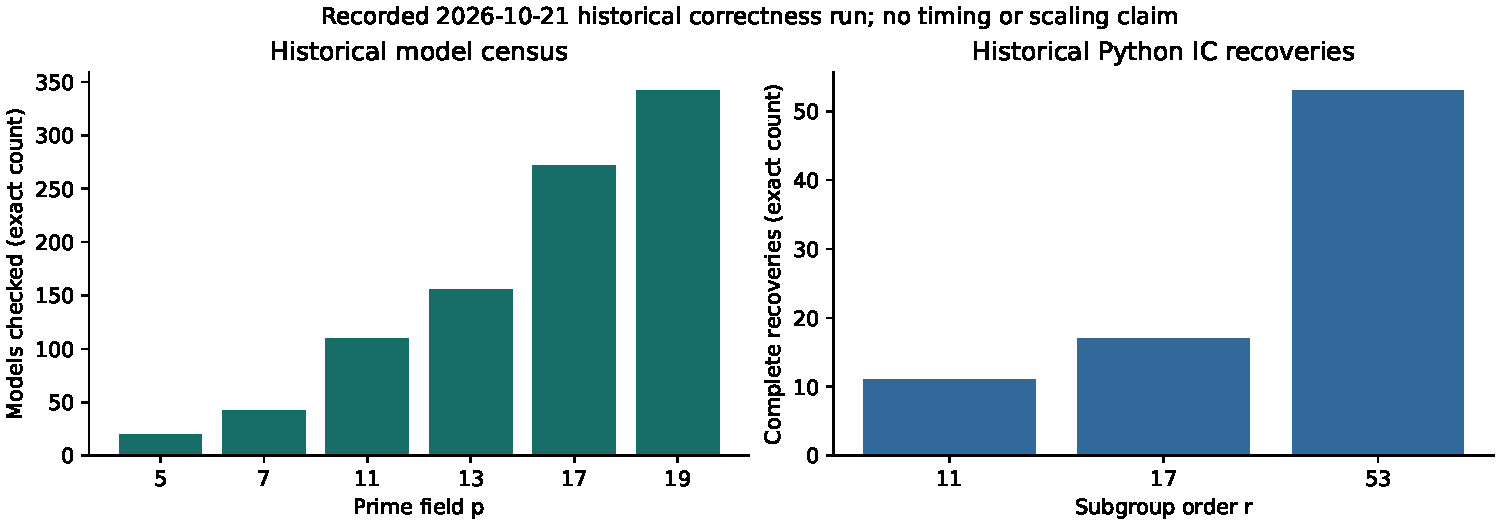
\includegraphics[width=\linewidth]{coverage.pdf}
\end{center}
\small Historical exact finite counts from \path{historical/results.json};
run started 2026-10-21 05:58:27 UTC. There is no statistical sampling error for
these counted domains, and no extrapolation is drawn.\normalsize

\textbf{Native audit observations.} The final audit at
\path{audits/run-20261021T064417Z/} checked all 12 internal hashes, three saved
full-rank IC matrices and their finite-field logarithm certificates, all 81
scalar-pairing identities, all 3,219 bilinearity identities, and the smooth and
anomalous twist point-count examples. Miller pairings and elliptic-curve scalar
identities were recomputed in C++. This verifies those finite certificates; it
does not independently witness the earlier Python process or its full census.

\textbf{Controls.} The native control run accepts the original snapshot, rejects
a modified experiment source, and rejects an algebraically false relation even
after that result file's checksum is updated. Expected rejections have nonzero
exit status. Transcripts are retained beside the native audit receipts.

\newpage
\section*{What the evidence establishes}
\begin{center}
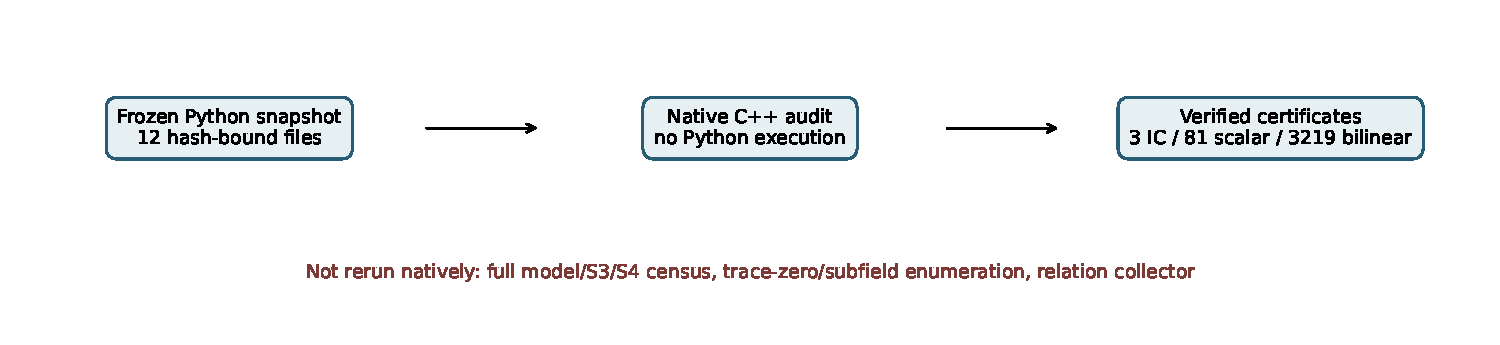
\includegraphics[width=\linewidth]{audit-scope.pdf}
\end{center}

The archived readable argument distinguishes the plus and minus Frobenius
eigenspaces. For a relation $R=A+B$, with $R,A$ rational on the original curve
and $B$ a sum of embedded twist-rational points, applying Frobenius gives
$R=A-B$, hence $2B=0$. The odd-primary twist contribution therefore vanishes.
The archive also retains a nonzero 2-torsion exception. These are statements
with specified hypotheses, not a prohibition of all twist-assisted methods.

The geometric summation-polynomial relation conditions are preserved by the
x-fixing quadratic-twist isomorphism over its splitting field. A shared odd
prime on a curve and its quadratic twist gives embedding degree two, enabling
the specific pairing reductions represented in the saved fixtures. A smooth
twist order does not force a smooth original order or a rational homomorphic
transfer. The native audit rechecks the two explicit point-count examples.

\section*{Requirements still open}
The full native census, trace-zero and subfield-descent enumeration, and relation
collection are not implemented here. The general written proofs have not been
formalized and checked in Lean, and the historical symbolic checks are not
registered identity certificates. General GHS construction and general ECDLP
hardness remain unestablished.

Conductor, Cargo/Rust, and Lean are absent from this execution environment.
The attempted Conductor and Cargo commands exited 127. No coordination
reservation, Rust library test pass, or Lean proof check is claimed. These are
tooling/implementation gaps, not mathematical obstructions. See
\path{validation/README.md} and \path{REQUIREMENTS.md}.

\section*{Reproduce and audit}
\begin{verbatim}
bash research/quadratic_twist_evidence_20261021/run-audit.sh
bash research/quadratic_twist_evidence_20261021/test-audit.sh
\end{verbatim}
Use fresh output directories; the scripts refuse to overwrite prior receipts.
The native auditor is \path{audit.cpp}. Its only library dependency is OpenSSL.
The report's Python file only lays out previously recorded values.

No benchmark, leaderboard, registry entry, or canonical IC/rho graph is promoted:
this import supplies no admissible cost or speedup row. The scoreboard,
leaderboard, progress timeline and lab browser remain unchanged for that reason.

\section*{Primary sources preserved by the historical study}
\begin{itemize}
\item Semaev, summation polynomials: \url{https://eprint.iacr.org/2004/031}.
\item Gorla--Massierer, trace-zero index calculus: \url{https://arxiv.org/abs/1405.1059}.
\item Menezes--Okamoto--Vanstone, pairing reduction:
\url{https://doi.org/10.1145/103418.103434}.
\item Gaudry--Hess--Smart, Weil descent:
\url{https://www.kantmath.de/publications/papers/weil_descent.pdf}.
\end{itemize}
\end{document}
